\section{The closed-loop market}\label{sec:model}

\subsection{Price formation}
Time is discrete with bars of length $\Delta$. Let $p_t$ be the price, $p^*_t=p^*_{t-1}+\xi_t$ the unobserved fundamental and $x_t=p_t-p^*_t$ the pricing error. Competitive dealers post aggregate depth $D>0$, so price impact is $\kappa=1/D$, and fundamental arbitrage removes a fraction $\kappa\varphi_f$ of the error each period. With algorithmic demand $u_t$ and liquidity noise, the pricing error follows
\begin{equation}\label{eq:price}
x_{t+1}=ax_t+\kappa u_t+w_{t+1},\qquad a=1-\kappa\varphi_f\in[0,1).
\end{equation}
Algorithmic cohorts trade $u_t=\sum_iq_iy_{i,t}$ with exponential memory $y_{i,t+1}=(1-\eta_i)y_{i,t}+\eta_ix_{t+1}$, a reduced form that arises when an adaptive desk updates its belief by steady-state Kalman filtering or regularized online gradient descent and maximizes expected continuation return $\beta_i y_{i,t}u_{i,t}$ minus quadratic execution cost $\tfrac12\lambda_{{\rm tc},i}u_{i,t}^2$ and inventory penalty $\tfrac12\gamma_{{\rm inv},i}I_{i,t}^2$ ($I_{i,t}=(1-\delta_{\rm inv})I_{i,t-1}+u_{i,t}$, $|I_{i,t}|\le\bar I_i$), yielding $u_{i,t}^*=q_iy_{i,t}-\psi_{{\rm inv},i}I_{i,t-1}$ with $q_i=\beta_i/(\lambda_{{\rm tc},i}+\gamma_{{\rm inv},i})$ and $\psi_{{\rm inv},i}=\gamma_{{\rm inv},i}(1-\delta_{\rm inv})/(\lambda_{{\rm tc},i}+\gamma_{{\rm inv},i})$ (\citealp{niroula2026}; this single-agent filtering-and-control rule is distinct from the joint dealer--trader equilibrium of Section~\ref{sec:equil}). The baseline equations set $\psi_{{\rm inv},i}=0$, the limit in which inventory holding penalties are small relative to execution costs ($\gamma_{{\rm inv},i}\ll\lambda_{{\rm tc},i}$) or inventory is reset at the bar horizon; Proposition~\ref{prop:inventory_S} below relaxes this and gives the closed-form summed response when cohorts carry inventory across bars with $\psi_{{\rm inv},i}>0$. Stacking $z_t=(x_t,y_{1,t},\ldots,y_{K,t})^\top$ gives $z_{t+1}=Jz_t+bw_{t+1}$, where $b=(1,\eta_1,\ldots,\eta_K)^\top$ because cohorts update on the same period's price (a unit of flow enters through $\kappa b$), and
\begin{equation}\label{eq:J}
J=\begin{pmatrix} a & \kappa q_1 & \cdots & \kappa q_K\\ \eta_1 a & 1-\eta_1+\eta_1\kappa q_1 & \cdots & \eta_1\kappa q_K\\ \vdots & & \ddots & \vdots\\ \eta_K a & \eta_K\kappa q_1 & \cdots & 1-\eta_K+\eta_K\kappa q_K\end{pmatrix}.
\end{equation}

\subsection{Stability and the role of depth}

\begin{proposition}[Stability with one cohort]\label{prop:jury}
With one cohort $(q,\eta)$ and $a=1-\kappa\varphi_f$, the market is Schur stable if and only if
\begin{equation}\label{eq:jury}
q<\varphi_f,\qquad \kappa<\frac{4-2\eta}{(2-\eta)\varphi_f-\eta q}\ \ \text{when}\ (2-\eta)\varphi_f>\eta q,\qquad |1-\kappa\varphi_f|(1-\eta)<1 .
\end{equation}
Higher impact $\kappa$ (thinner depth) lowers price persistence $a$; feedback is destabilizing only when cohort aggressiveness $q$ reaches the arbitrage strength $\varphi_f$.
\end{proposition}

The condition $q<\varphi_f$ is the familiar statement that momentum demand must be weaker than value arbitrage. The upper bound on $\kappa$ rules out oscillatory instability when the book is very thin.

\subsection{What an observer can use}

The companion paper shows that prices identify only the merged rate--weight measure $M=\sum_iq_i\eta_i\delta_{1-\eta_i}$ of the cohorts. A pre-trade control must therefore depend on the market only through objects that are the same for every cohort representation of $M$.

\begin{proposition}[Input--output invariance]\label{prop:invariance}
Two populations with the same merged measure generate the same transfer function $H(z)=\sum_kg_kz^{-k}=\kappa z/[z-a-\kappa G(z)]$, $G(z)=\sum_iq_i\eta_iz/(z-1+\eta_i)$, and the same impulse coefficients $g_k=\kappa\,c_{\rm price}^\top J^kb$ for every $k\ge0$. Under any invertible change of state coordinates $z\mapsto Tz$, the Euclidean gain $\|CT^{-1}(TJT^{-1})^k\|_2$ depends on $T$, whereas the price path
\[
\Delta p_{t+k}=\sum_{j\ge1}g_{k-1+j}u_{t-j}+\sum_{m=0}^{k-1}g_{k-1-m}u_{t+m}
\]
and its worst case over $\|u\|_\infty\le\bar u$ depend only on $\{g_k\}$ and are invariant to both $T$ and cohort splitting.
\end{proposition}

Numerically, splitting a cohort of 1{,}000 random economies into two with the same memory rate leaves every impulse coefficient unchanged up to rounding ($\max_k|g_k(\mathcal E^A)-g_k(\mathcal E^B)|\le2.5\times10^{-12}$ over 200 lags; \texttt{recompute\_oct20.py}). Proposition~\ref{prop:invariance} is the reason we build the guard on impulse coefficients and avoid state norms in latent coordinates. When a state norm is needed, we fix units by observable calm-market innovation standard deviations, which is what makes the spot statistic of Section~\ref{sec:spot} unit-free.

\begin{proposition}[Summed response with carried cohort inventory]\label{prop:inventory_S}
Suppose each cohort $i$ carries inventory $I_{i,t}=(1-\delta_{\rm inv})I_{i,t-1}+u_{i,t}$ with $\delta_{\rm inv}\in(0,1]$ and submits order flow $u_{i,t}=q_i y_{i,t}-\psi_i I_{i,t-1}$ with $q_i\ge0$ and $\psi_i\ge0$. Then:
\begin{enumerate}[label=(\roman*)]
\item The closed-loop transfer function from a flow impulse to price is $H_{\rm inv}(z)=\kappa z/\bigl[z-a-\kappa G_{\rm inv}(z)\bigr]$ with
\[
G_{\rm inv}(z)=\sum_{i=1}^K \frac{q_i\eta_i z(z-1+\delta_{\rm inv})}{(z-1+\eta_i)(z-1+\delta_{\rm inv}+\psi_i)},
\]
which is invariant to splitting any cohort that shares $(\eta_i,\psi_i)$. Whenever the augmented state matrix is Schur stable, the signed cumulative price response is
\begin{equation}\label{eq:Sinv}
S(\psi)=\sum_{t=0}^\infty h_t(\psi)=H_{\rm inv}(1)=\frac{\kappa}{1-a-\kappa\Phi_{\rm eff}(\psi)},\qquad \Phi_{\rm eff}(\psi)\equiv\sum_{i=1}^K\frac{\delta_{\rm inv}}{\delta_{\rm inv}+\psi_i}\,q_i\le\Phi.
\end{equation}
\item If $0\le\psi_i\le 1-\delta_{\rm inv}$ and $\delta_{\rm inv}\ge\eta_i$ for each $i$ and $a+\kappa\Phi_{\rm eff}(\psi)<1$, every open-loop feedback tap $k_m(\psi)$ and hence every closed-loop impulse coefficient $h_t(\psi)$ is nonnegative, so the worst-case $\ell_1$ gain equals the signed sum, $\|h(\psi)\|_1=\sum_{t=0}^\infty |h_t(\psi)|=S(\psi)$. When $\psi_i$ is large enough that inventory payback reverses the sign of late taps, $\|h(\psi)\|_1>S(\psi)$.
\end{enumerate}
\end{proposition}

Inventory mean-reversion $\psi_i>0$ acts as an automatic stabilizer that attenuates each cohort's long-run feedback weight from $q_i$ to $\frac{\delta_{\rm inv}}{\delta_{\rm inv}+\psi_i}q_i$ (across 500 random stable economies \eqref{eq:Sinv} matches the simulated state-space impulse sum to $1.78\times10^{-15}$, and in the monotone regime $\|h(\psi)\|_1=S(\psi)$ to $1.78\times10^{-15}$, reducing $S$ from $2.7778$ at $\psi=0$ to $2.5000$ at the calibrated worked example; in the sign-reversal regime $\|h(\psi)\|_1=2.0960>S(\psi)=1.7241$; \texttt{recompute\_p2\_step2\_theory.py}).

\begin{proposition}[Quote cost of ambiguity]\label{prop:ambig}
For a one-unit ticket with adverse mark $Z_\theta\sim N(\mu_\theta,\sigma_\theta^2)$ and a CARA dealer with risk aversion $\gamma$, let $c_\theta=\mu_\theta+\gamma\sigma_\theta^2/2$. Under competition with zero robust certainty equivalent, the informed quote is $c_{\theta_0}$ and the ambiguous quote $\sup_\theta c_\theta$; with inverse demand $(V_0-V)/b$ and marginal cost $c$, raising an interior quote from $s_0$ by $\Delta$ costs $b(s_0-c)\Delta+\tfrac b2\Delta^2$ in surplus.
\end{proposition}

Ambiguity about the algorithms is costly only when it changes the worst relevant cost. A guard that bounds worst-case transient exposure can therefore narrow the ambiguity premium; whether it does in a real market is an empirical question we do not answer here.

\subsection{Discussion of the assumptions}

\paragraph{Linearity and small shocks.} All dynamics are linear. This is the right approximation for the transient response to flow shocks of ordinary size, which is what a pre-trade control must bound one step ahead; it is not a model of regime changes such as exchange outages, where nonlinear liquidity withdrawal dominates.

\paragraph{One book, one asset.} Sections~\ref{sec:t6}--\ref{sec:guard} treat a single instrument; Proposition~\ref{prop:multi} shows how directed cross-impact enlarges transient gains in a network. Cross-margined portfolios need the multi-asset operator, which we leave to future work.

\paragraph{Bounded shocks.} The guard bounds losses for shocks in a declared envelope. Choosing the envelope is a risk-management decision; a larger envelope trades admitted flow for safety. The theorems hold for any envelope, and the empirical work does not depend on it.

\paragraph{Observables.} Every input to the guard (impulse coefficients, an operator estimate and its confidence radius, inventory and margin) is observable to a dealer or venue. Nothing requires the identities or memory parameters of the algorithms.

\section{Spectral stability is not solvency}\label{sec:radius}

\begin{theorem}[Safe radius, Kreiss bounds and the failure of the spectral radius]\label{thm:radius}
Let $z_t=J^tz_0$ with $\rho(J)<1$, loss budget $B>0$ and loss output $C$.
\begin{enumerate}[label=(\roman*)]
\item The largest initial-state radius with $\sup_t\|CJ^tz_0\|_2\le B$ for every $\|z_0\|_2\le r$ is
\begin{equation}\label{eq:rexact}
r^*_{\rm exact}=\frac{B}{M_C},\qquad M_C\equiv\sup_{t\ge0}\|CJ^t\|_2 .
\end{equation}
\item With $C=I$ and the Kreiss constant $\mathcal K(J)=\sup_{|z|>1}(|z|-1)\|(zI-J)^{-1}\|_2$, the Kreiss matrix theorem gives $\mathcal K(J)\le\sup_t\|J^t\|_2\le e\,n\,\mathcal K(J)$ for $J\in\R^{n\times n}$, hence
\begin{equation}\label{eq:kreiss}
\frac{B}{e\,n\,\mathcal K(J)}\;\le\;r^*_{\rm exact}\;\le\;\frac{B}{\mathcal K(J)} .
\end{equation}
\item For any $\rho\in(0,1)$ and any $B>0$ there is a family $J_\theta$ with $\rho(J_\theta)=\rho$ for all $\theta$ and an output $C=(1,0)$ such that $r^*_{\rm exact}(J_\theta)\to0$ as $\theta\to\infty$.
\end{enumerate}
\end{theorem}

Table~\ref{tab:kreiss} illustrates the theorem for $J_\theta=\begin{psmallmatrix}0.8&\theta\\0&0.4\end{psmallmatrix}$: the spectral radius is $0.8$ throughout, while the price-row gain rises from 1 to 120 and the safe radius falls by the same factor. The Kreiss constant tracks the gain within the factor $en$.

\begin{table}[t]\centering\small
\begin{threeparttable}
\caption{Safe radius and Kreiss bounds at a fixed spectral radius}\label{tab:kreiss}
\begin{tabular}{rccccc}
\toprule
$\theta$ & $\rho(J_\theta)$ & $M_C$ (price row) & $\sup_t\|J_\theta^t\|$ & $\mathcal K(J_\theta)$ & $r^*_{\rm exact}$ ($B=1$)\\
\midrule
0 & 0.8 & 1.00 & 1.00 & 1.00 & 1.000\\
1 & 0.8 & 1.36 & 1.37 & 1.06 & 0.735\\
5 & 0.8 & 6.03 & 6.04 & 3.43 & 0.166\\
20 & 0.8 & 24.01 & 24.01 & 13.42 & 0.042\\
100 & 0.8 & 120.00 & 120.00 & 66.99 & 0.008\\
\bottomrule
\end{tabular}
\begin{tablenotes}\footnotesize\item $J_\theta=\begin{psmallmatrix}0.8&\theta\\0&0.4\end{psmallmatrix}$; Kreiss constant by grid search over $|z|>1$. \end{tablenotes}
\end{threeparttable}
\end{table}

The theorem concerns a specified initial-state ball and output norm. Changing state coordinates changes the disturbance set, so latent-state units cannot be read as monetary losses; this is why Section~\ref{sec:guard} works with input--output gains instead.

\paragraph{Spectral blindness.} The companion paper shows more: for any eigenvalues $0<\lambda_2<\lambda_1<1$, one-step price variance and sufficiently large stationary price variance, there are two-state markets sharing all three quantities whose worst-case transient gain is arbitrarily large \citep[spectral-blindness theorem]{niroula2026}, so neither eigenvalue nor volatility monitors bound transient loss.

At $\lambda=(0.8,0.7)$ with one-step variance 1 and stationary variance 5, the gain is $1.77$, $5.10$, $16.95$, $50.85$ and $169.50$ as the off-diagonal coupling rises from 1 to 100. Figure~\ref{fig:pseudo} shows the geometry for a constructed matrix with spectral radius $0.5$: its pseudospectra cross the unit circle, and the price-row gain grows with the coupling before decaying.

\begin{figure}[t]\centering
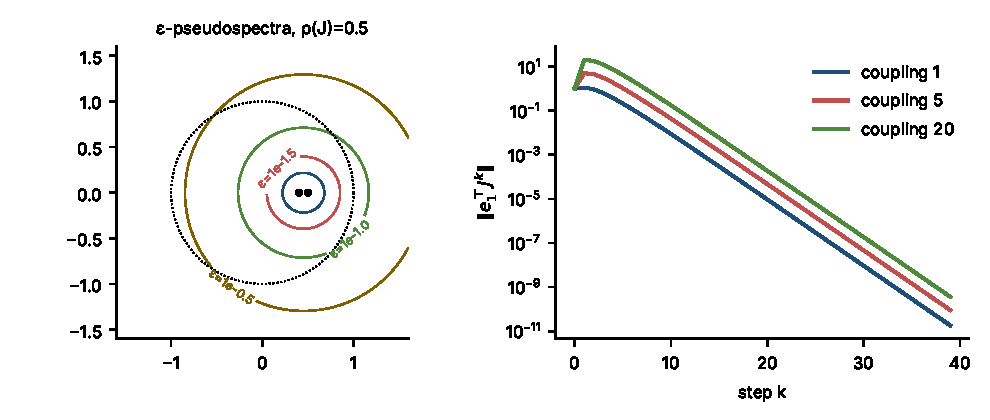
\includegraphics[width=0.95\textwidth]{figs/fig_pseudo.pdf}
\caption{Left: $\varepsilon$-pseudospectra of $J=\begin{psmallmatrix}0.5&5\\0&0.4\end{psmallmatrix}$; the eigenvalues (dots) are well inside the unit circle (dotted), but the $\varepsilon=10^{-1}$ contour reaches beyond it. Right: price-row gain $\|e_1^\top J^k\|$ for couplings 1, 5 and 20.}\label{fig:pseudo}
\end{figure}

\paragraph{No amplification without depth.} In the cohort economy \eqref{eq:J} with nonnegative weights and $\rho(J)<1$, the price impulse response is a nonnegative mixture of decaying exponentials with total weight $\kappa$; it is completely monotone and peaks at the direct impact \citep[positive-geometry lemma]{niroula2026}.

This is a negative result with a positive use. The cohort matrix \eqref{eq:J} is non-normal, yet its price output never amplifies. Non-normality alone is not sufficient for price overshoot. Its necessity for Euclidean state-norm growth of a normal-contraction comparison does not extend to arbitrary scalar input-output overshoot. The no-overshoot result here uses the positive-cohort structure. Section~\ref{sec:t6} shows that depth depletion does.

\subsection{Multi-asset coupling}

Market makers trade many correlated instruments. Let $x_t\in\R^d$ be pricing errors and $u_t\in\R^d$ flows, with $x_{t+1}=Ax_t+Ku_t+w_{t+1}$, $A={\rm diag}(a_1,\ldots,a_d)$, a cross-impact matrix $K$, and momentum flow $y_{t+1}=(I-H)y_t+Hx_{t+1}$, $u_t=Qy_t$. The stacked Jacobian is
\begin{equation}\label{eq:Jmulti}
J_{\rm multi}=\begin{pmatrix}A&KQ\\ HA&I-H+HKQ\end{pmatrix}\in\R^{2d\times2d}.
\end{equation}

\begin{proposition}[Directed cross-impact shrinks the safe radius]\label{prop:multi}
Suppose a leader--satellite structure ($K_{12}=0$, $K_{21}\ge0$) with $A,Q,K\ge0$ entrywise, $H\in(0,1)^d$, stable diagonal blocks and a fixed output $C\ge0$. Let $J_{\rm diag}$ be the decoupled Jacobian with $K_{21}=0$. Then every power $J_{\rm multi}^t$ is entrywise non-decreasing in $K_{21}$, so $M_C(J_{\rm multi})\ge M_C(J_{\rm diag})$ and $r^*_{\rm exact}(J_{\rm multi})\le r^*_{\rm exact}(J_{\rm diag})$; likewise $\mathcal K(J_{\rm multi})\ge\mathcal K(J_{\rm diag})$.
\end{proposition}

The proposition concerns nonnegative downstream coupling under a fixed output and shock set. Hedged or signed monetary outputs need separate treatment, and the size of the effect requires an empirical calibration we do not provide. Persistence and transient amplification are nevertheless different things: in a network of identical cohort economies coupled by symmetric nonnegative cross-impact, which stays symmetric in suitable coordinates, cross-impact of $0.05$ raises the spectral radius from $0.822$ ($d=1$) to $0.973$ ($d=10$) while the Kreiss constant stays at one (\texttt{recompute\_oct20.py}). Directed coupling, as in Proposition~\ref{prop:multi}, is what turns persistence into amplification.
